\documentclass{report}
%\usepackage{includegraphicx}
\usepackage{sydewkrpt}
\usepackage{longtable}
\usepackage{array}
\usepackage{ragged2e}
\usepackage{amsmath}
\usepackage{amssymb}
\usepackage[toc]{glossaries}
\setcounter{secnumdepth}{5}
\setcounter{tocdepth}{5}
\DeclareMathOperator*{\argmin}{\arg\!\min}
\DeclareMathOperator*{\argmax}{\arg\!\max}
\newcolumntype{P}[1]{>{\RaggedRight\hspace{0pt}}p{#1}}

\makeglossaries

%%%%%%%%%%%%%%%%%%%%%%%%%%%%
%%%    Begin Document    %%%
%%%%%%%%%%%%%%%%%%%%%%%%%%%%
\begin{document}
\pagenumbering{roman}

\waterlootitle{SYDE 462: Spring Term Final Report}{
  Group 2: Relay \\
  Adaptive Traffic Control Framework
}{
  Alex Huras -- 20344660\\
  D. Scott Neil -- 20349210\\
  Myles Tan -- 20349217\\
  Riley Donelson -- 20342815\\
  }

\dotableofcontents

\newpage

\chapter*{Glossary of Terms}
\begin{description}
\item[Angular.js] A client-side JavaScript Framework.
\item[Backbone.js] A client-side JavaScript Framework.
\item[DOJO] A client-side Javascvript Framework.
\item[JavaScript MVC] A client-side JavaScript Framework.
\item[jQuery] A client-side JavaScript Utility Library.
\item[Underscore.js] A client-side JavaScript Utility Library.
\end{description}


\newpage
\doublespacing
\pagenumbering{arabic}

\chapter{Background Information}
\setlength{\parindent}{1cm}

\newpage

\chapter{Engineering Design}

\section{Front End}

\subsection{Design Research}
The Front End design process began with a Research phase, intended to provide a clear picture of the industry and potential users.
This was accomplished through a User Study including interviews with industry experts, the gathering of Functional Requirements and Use Cases for the Relay Interface, and a detailed look at Information Architecture methods to best display the required data.

\subsubsection{User Study}
With intentions to create a product suitable for both Traffic Engineers and consumers, the Engineering Design process for the Front End Relay application began with a User Study conducted towards both types of ideal product users.
The study consisted of industry research, investigating existing traffic visualization solutions, and interviews conducted with experts to gather their insights on users, as well as their knowledge of the industry and how a solution such as Relay may fit into the product landscape. 

Industry Research was conducted through an analysis of the State of the Art in traffic visualization products and solutions. 
These product offerings were found to be primitive in type of data available, generally providing a boolean or three-stage metric of traffic/no-traffic, or traffic/light-traffic/no-traffic.
Products where these interfaces were found include Apple Maps and Google Maps, where the target audience is the general public. 
This finding was important in guiding the consumer-focused aspect of the Relay Interface, as it emphasized the need for simplicity and salience in the design.
Other traffic-related software, on the Traffic Engineer side, includes simulation environments such as PTV VisSim.
Findings from this software were quite the opposite from the consumer-focused applications, as the simulation environment was very heavily loaded with information, features, and required a great deal of time to learn to use.
Even with such elaborate software suites available, the user is still limited to a model/simulation of the actual scenarios and data they may encounter in the real world.
True, accurate, live traffic interfaces are still relatively primitive and consumer-focused, meaning that in-depth intersection data simply is not readily available in an online application.
Experiencing both extremes of existing software opened up an important area for Relay to be focused on - creating a balanced program that will not overload beginner or light-use users, such as the average route-planning consumer, while being able to supply the necessary data, insight, and control that a Traffic Engineer would require to effectively monitor their network and empower the work that they do.
With this in mind, the team conducted three interviews with experts in the traffic engineering industry, to gather their insight into the matter.

The first expert interview was conducted with Marc Tan from IBI Group in Toronto.
The transcript for this interview is available in Appendix \ref{interview-marc}. 
The goal of this interview was to understand the nuances of what a Traffic Engineer does, what their needs are in an interface, and how their role may change given an adaptive control system.
Marc enlightened the team on the three main roles that exist for those involved in traffic network planning and execution.
These roles are the Traffic Engineers - who draw up signal timing plans, Technical Staff - who work in control centres changing signal timing plans, usually under the direction/instruction of a traffic engineer, and Technicians - who often hard code timings or fall back plans out in the field.
It was identified that Traffic Engineers are found to be drawing up signal timing plans less and less as adaptive technology progresses forward.
\begin{quote}
``As systems become adaptive, the goal of the traffic engineer is to more so calibrate and set up the existing conditions of the network rather than drawing up particular definitive second by second timings.''
\end{quote}
This quote from Mr. Tan was important in the development of functional requirements directed at Traffic Engineers, as their goals in the context of an adaptive system are shown to be different from those in non-adaptive systems.
With a need to calibrate and set up existing conditions of the network, a strong emphasis can be placed on being able to monitor these network conditions, validating the need for a well-designed data interface.
This interview was also important in gathering a more holistic view of the concerns of a traffic engineer.
\begin{quote}
``Now we don't just look at traffic; pedestrian and cyclist volumes also play a major role in determining timings.
Other things to consider are the capabilities of the existing system, and the communication channels available (i.e. are the traffic signals connected to a central system, can we change them from a central system, are there other factors at play (special timings for transit, cyclists, pedestrians, etc.), is there an adaptive system.''
\end{quote}
From this, the strong need to consider everything that goes on at an intersection, not just vehicular traffic, is evident in informing the decisions that traffic engineers need to make.
The ability to make informed decisions is based on the available data, which places emphasis on the need for accurate data acquisition technology at intersections, such as image processing techniques to gather data on pedestrians, cyclists, and other actors that may not be detected by the typical loop sensors often implanted into roads.
Given appropriate data acquisition at intersections, it is evident that the display of that information is critical in an interface to be used by Traffic Engineers.

The second interview was conducted with Peter Kelley of Paradigm Transportation.
A transcript for this interview is included in Appendix \ref{interview-peter}.
This interview went into detail regarding the specific metrics of interest that a Traffic Engineer may monitor, on both system-wide and per-intersection scale.
Mr. Kelley was helpful in identifying the need to display the overall experienced delay in the network, and the importance of knowing the signal timing plans and volume of vehicles moving through the network.
In the case of an adaptive system, having a window into its decision-making process and predictions is critical in understanding why the network is behaving the way that it is.
He was able to identify certain edge cases where existing traffic solutions often fail - such as the precedence that emergency vehicles take over the network, and the difficulty that a pre-set timing system has recovering from such an anomaly.
\begin{quote}
``A big problem for this is emergency vehicles that can control the signal to get priority, having the signals get back on cycle can take a while and overall negatively impacts traffic flow.''
\end{quote}
Being able to spot abnormal situations at an intersection gave insight into the need for a metric displaying the status of an intersection, where it may be experiencing some sort of unusually long delay, a power outage, an accident, etc.
While an adaptive system will be able to intelligently route traffic around such an anomaly and quickly get back into a regular timing scheme, it is still important to be able to alert the engineer of situations as they arise, as well as to provide a look-back at a log or history of activity at an intersection to try and detect any patterns that could influence re-programming.
On an individual-intersection basis, Mr. Kelley identified issues with the way current solutions assign minimum amounts of green time in certain directions at peak hours, and how this creates problems when such patterns change. 
Being able to provide protected movements when no one is at the intersection, or at least not in individual directions, is a major bonus that adaptive systems offer for mitigating these peak hour concerns. 
Additional information that Traffic Engineers need to monitor were identified to include turn counts, volume, an overall Level of Service metric, and more.
\begin{quote}
``The information we like to know about a single intersection is the turning movement counts, the delay of the approaches (north, south, east, west), the queue lengths of vehicles, and the volume/capacity ratio. These all serve as a means to determine the Level of Service of an intersection.''
\end{quote}

The final interview was conducted with David Hillis from Miovision in Kitchener.
This interview provided a clear look into the traffic engineering landscape as a whole, detailing information on existing solutions, the needs/goals/desires of a traffic engineer, and some of the roadblocks and challenges that Miovision has faced in developing an adaptive traffic control system of their own.
Firstly, Mr. Hillis identified some limiting factors for adaptive systems - budget being the biggest deterrent for many governments and municipalities.
Implementing new technology, particularly expensive new technology, in infrastructure can be a major challenge, as there are many concerns such as fault tolerance, safety, and cost that must be held to an extremely high standard.

Another interesting point discussed was the effect of psychological factors on drivers, identifying that predictability on a route often trumps true efficiency.
An individual driver wants to be able to optimize and ``out-smart'' the lights on their route.
When the timings on the route itself are changing and optimizing for the overall benefit of the network, as is the case in an adaptive system, individual drivers may believe they are not getting a great service as they get many green lights one day, and many red lights the next.
Understanding the psychological factors at play is important in gaining a truly holistic understanding of the traffic system, and must be taken into consideration when designing an interface where consumers and traffic engineers must get a maximal benefit.

Mr. Hillis also identified the truly primitive nature of the underlying traffic control technology, and the way that timing plans are often updated.
He discussed that people will often call in to complain about a particular intersection, or to alert the city that an intersection is down or there is a power outage.
The data gathered at intersections currently has no convenient way of being exported and processed, as many locations require a technician or engineer to plug in a monitor to view the workings of a particular intersection.
The data that was identified as important includes the phase of the lights (i.e. which direction is green, red, is there an advanced green, etc.), and the overall delay/queue length at an intersection and across the network.
For the interface, Mr. Hillis advised that users should be given a sense of control and purpose, with the ability to tweak things and make changes as necessary, while exposing as much data as possible.
By providing an interface that meets these needs, both consumers and traffic engineers will be empowered to make better decisions on their driving and route-planning habits, as well as on the work that they do surrounding the behaviour of the traffic network.

\subsubsection{Functional Requirements}
With the insights gathered through researching industry solutions and state-of-the-art traffic interfaces, as well as through conversations with traffic engineering experts, a detailed set of Functional Requirements and Use Cases for the Relay Interface were compiled. 
In the following tables, the shorthand ``TE'' will be used to denote Traffic Engineer, and ``Network'' refers to the collection of intersections and roads which the traffic control system controls.
The specific area that a requirement is related to is numbered, while the requirements themselves follow a letter-based enumeration scheme.
Particular requirements will be referred to by their numerical and letter positioning, e.g. Requirement 2b.

\begin{enumerate}
  \item Network
  \begin{enumerate}
    \item The TE should be able to see all of the intersections in the network on a map.
    \item The TE should be able to see a list of all of the intersections in the network.
    \item The TE should be able to see the performance metrics of the network.
    \item The TE should be able to see the history of the performance metrics for the network.
  \end{enumerate}
  \item Intersections
  \begin{enumerate}
    \item The TE should be able to see the status of all of the intersections in the network.
    \item The TE should be able to see basic performance information about all of the intersections in the network.
    \item The TE should be able to search for an intersection in the network and see the details of the intersection.
    \item The user should be able to see an intersection's position on a map.
    \item The user should be able to see basic information about the intersection.
    \begin{enumerate}
    	\item Title
	\item Type of intersection (major, minor, etc.)
	\item Geographic co-ordinates
    \end{enumerate}
    \item The user should be able to see the status of the intersection.
    \item The user should be able to see the signal state of the intersection.
    \item The user should be able to see current performance metrics of the intersection.
    \item The user should be able to see the history of the intersection's performance.
  \end{enumerate}
  \item Roads
  \begin{enumerate}
    \item The TE should be able to see the status of all of the roads in the network.
    \item The TE should be able to see basic performance information about all of the roads in the network.
    \item The TE should be able to search for a road in the network and see the details of the road.
    \item The user should be able to see the road on a map.
    \item The user should be able to see basic information about the road.
    \begin{enumerate}
    	\item Type of road
	\item Width of road
	\item Speed limit
    \end{enumerate}
    \item The user should be able to see the current performance of the road.
    \item The user should be able to see the history of the intersection's performance.
  \end{enumerate}
\end{enumerate}

Following the compilation of these Functional Requirements, a series of Use Cases, as outlined in Tables \ref{use-case-1} - \ref{use-case-8} were created to provide a better sense of particular tasks and situations users may often be in, to help promote a more user centred approach to the design of the Relay Interface.

\begin{table}[htbp]
\begin{centering}
    \begin{tabular}{| p{7cm} | p{7cm} |}
    \hline
    User    & Interface   \\ \hline
    User types in the Relay URL    &     The application loads to show the loading screen    \\ \hline
    ~      & When the loading is done, the application displays a map of the network. The map highlights controlled roads and intersections. \\ \hline
     User monitors the map for activity and high-level performance. & ~          \\ \hline
    \end{tabular}
    \caption {Use Case 1: User monitors network map.}
    \label{use-case-1}
   \end{centering}
\end{table}

\begin{table}[htbp]
\begin{centering}
    \begin{tabular}{| p{7cm} | p{7cm} |}
    \hline
    User    & Interface   \\ \hline
    User types in the Relay URL    &     The application loads to show the loading screen    \\ \hline
    ~      & When the loading is done, the application displays a map of the network. The map highlights controlled roads and intersections. \\ \hline
     User selects the ``intersections'' tab  &    Application switches to showing the list of intersections.          \\ \hline
    The user monitors the list for activity.   &    \\ \hline
    \end{tabular}
    \caption {Use Case 2: User monitors intersection list.}
    \label{use-case-2}
   \end{centering}
\end{table}

\begin{table}[htbp]
\begin{centering}
    \begin{tabular}{| p{7cm} | p{7cm} |}
    \hline
    User    & Interface   \\ \hline
    User types in the Relay URL    &     The application loads to show the loading screen    \\ \hline
    ~      & When the loading is done, the application displays a map of the network. The map highlights controlled roads and intersections. \\ \hline
     User selects the ``roads'' tab  &    Application switches to showing the list of roads.          \\ \hline
    The user monitors the list for activity.   &    \\ \hline
    \end{tabular}
    \caption {Use Case 3: User monitors road list.}
    \label{use-case-3}
   \end{centering}
\end{table}

\begin{table}[htbp]
\begin{centering}
    \begin{tabular}{| p{7cm} | p{7cm} |}
    \hline
    User    & Interface   \\ \hline
    User types in the Relay URL    &     The application loads to show the loading screen    \\ \hline
    ~      & When the loading is done, the application displays a map of the network. The map highlights controlled roads and intersections. \\ \hline
     User selects the ``intersections'' tab  &    Application switches to showing the list of roads.          \\ \hline
    The user types the name of an intersection into the search bar.   &   The list filters real-time to show the list of intersections which match the search text.   \\ \hline
    The user locates the correct intersection     &     The row contains basic information about the intersection. \\ \hline
    \end{tabular}
    \caption {Use Case 4: User searches for an intersection.}
    \label{use-case-4}
   \end{centering}
\end{table}

\begin{table}[htbp]
\begin{centering}
    \begin{tabular}{| p{7cm} | p{7cm} |}
    \hline
    User    & Interface   \\ \hline
    User types in the Relay URL    &     The application loads to show the loading screen    \\ \hline
    ~      & When the loading is done, the application displays a map of the network. The map highlights controlled roads and intersections. \\ \hline
     User selects the ``roads'' tab  &    Application switches to showing the list of roads.          \\ \hline
    The user types the name of a road into the search bar.   &   The list filters real-time to show the list of intersections which match the search text.   \\ \hline
    The user locates the correct road     &     The row contains basic information about the road. \\ \hline
    \end{tabular}
    \caption {Use Case 5: User searches for a road.}
    \label{use-case-5}
   \end{centering}
\end{table}

\begin{table}[htbp]
\begin{centering}
    \begin{tabular}{| p{7cm} | p{7cm} |}
    \hline
    User    & Interface   \\ \hline
    User types in the Relay URL    &     The application loads to show the loading screen    \\ \hline
    ~      & When the loading is done, the application displays a map of the network. The map highlights controlled roads and intersections. \\ \hline
     User expands the details tab  &   The details tab expands to fill the right-hand side of the map. The user can see detailed performance metrics of the network. The user can see overview statistics about the roads in the network. The user can see overview statistics about the intersections in the network. The user can see historical information about the performance of the network. The user can see predictions of the performance of the network.          \\ \hline
    \end{tabular}
    \caption {Use Case 6: User inspects network details.}
    \label{use-case-6}
   \end{centering}
\end{table}

\begin{table}[htbp]
\begin{centering}
    \begin{tabular}{| p{7cm} | p{7cm} |}
    \hline
    User    & Interface   \\ \hline
    User types in the Relay URL    &     The application loads to show the loading screen    \\ \hline
    ~      & When the loading is done, the application displays a map of the network. The map highlights controlled roads and intersections. \\ \hline
     The user selects an intersection from the map  &   The intersection that was selected is highlighted on the map. A popup appears with basic information about the intersection. The user can see the current status of the intersection. The user can see the signal state of the intersection. The user can see the current performance level of the intersection. The user can see the current bias vector of the intersection.          \\ \hline
     The user selects ``show more'' in the intersection popup.     &    The popup closes and the details panel expands from the side of the screen with detailed information about the intersection. Application shows the current status of the intersection. Application shows the signal state of the intersection. Application shows the current performance level of the intersection. Application shows the current bias vector of the intersection. Application shows the flow biases for each direction in the intersection. Application shows performance and volume histories for the intersection. Application shows predictions for the intersection. \\ \hline
    \end{tabular}
    \caption {Use Case 7: User inspects intersection details.}
    \label{use-case-7}
   \end{centering}
\end{table}

\begin{table}[htbp]
\begin{centering}
    \begin{tabular}{| p{7cm} | p{7cm} |}
    \hline
    User    & Interface   \\ \hline
    User types in the Relay URL    &     The application loads to show the loading screen    \\ \hline
    ~      & When the loading is done, the application displays a map of the network. The map highlights controlled roads and intersections. \\ \hline
     User selects the ``road'' tab  &   Application switches to showing the list of roads.          \\ \hline
     The user types the name of an road into the search bar.     &    The list filters real-time to show the list of roads which match the search text.           \\ \hline
     The user locates the correct road.    &    The row contains basic information about the intersection.    \\ \hline
     The user selects the details icon on the row.     &     The detail panel appears from the right hand side of the page containing detailed information about the road. The user can see the road's profile. The use can see the performance level of the road. The user can see the speed and volume levels of the road. The user can see the historical volume, speed, and performance levels of the road. The user can see the performance, volume, and speed predictions for the road.     \\ \hline
    \end{tabular}
    \caption {Use Case 8: User inspects road details.}
    \label{use-case-8}
   \end{centering}
\end{table}

These requirements and use cases, resulting from the User Study outlined above and group brainstorming and ideation sessions, lay the foundations for the Relay Interface - the design of which is explained in detail in the Design Process section.
Prior to embarking on the Design Process for the Relay Interface however, further research and planning was done towards the information architecture of the application, given that it relies so heavily on the clear presentation of data.
The next section outlines the research process involved in gathering knowledge and ideas for the presentation and visualization of data in the Relay Interface.

\subsubsection{Information Architecture}
Research into information architecture began with a look at some existing academic literature on data visualization, particularly that involving glyph-based illustrations.
Given the requirements, it is evident that some complex data will need to be displayed in the application, particularly in a clean and understandable manner.
Glyph-based visualization works well in these scenarios, as patterns of multivariate data involving more than two attribute dimensions can often be more readily perceived in the context of a spatial relationship \cite{borgo2012glyph}.
The following table in Figure \ref{fig:glyphs} outlines six commonly used glyph types, breaking down their temporal encoding, ranked data value and issues that arise with each in situations of high data density \cite{fuchs2013evaluation}.

\begin{figure}[htbp!]
  \begin{centering}
    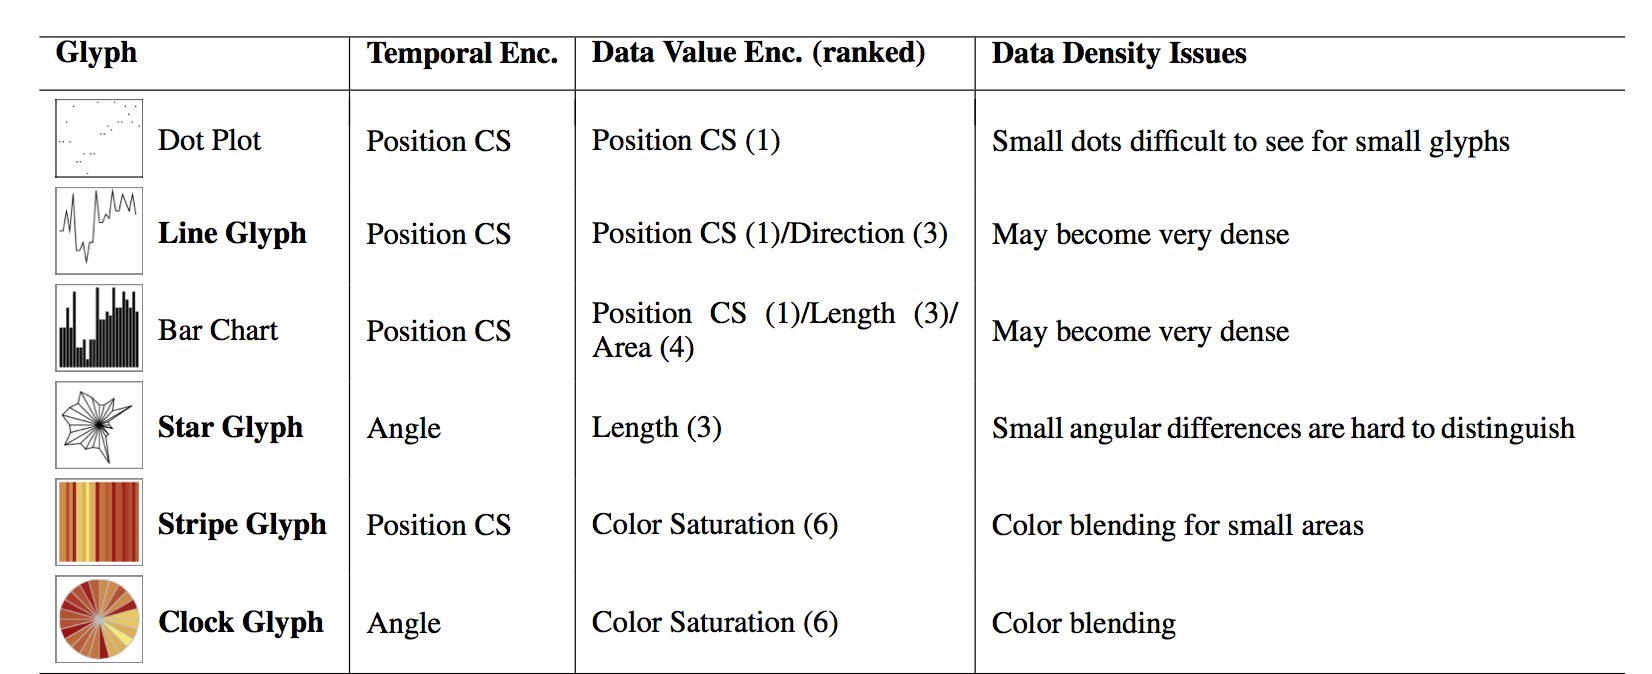
\includegraphics[scale=0.27]{figures/glyph_table.png}
    \caption{Common glyph types and their description.}
    \label{fig:glyphs}
  \end{centering}
\end{figure}

As can be seen in Figure \ref{fig:glyphs}, each common glyph type has their relative strengths and weaknesses.
The important considerations when bringing these visualizations into the Relay Interface is to carefully evaluate the data being presented, and to maximize the saliency of said data, while minimizing issues that may arise with the visualization at at size or density.

Upon making such decisions for the visualization of data, careful planning must be done to place data in locations on the screen and within the application such that the user need not search extensively to find it.
Certain data given by the requirements will be best served on the map, where the context of location and spatial relativity is important.
Other data may be better suited for presentation off of the map, perhaps in a dashboard or modular window setting.
Situations where the context of a single location is important, or in a list-based visualization environment may be areas where data is better suited to be shown away from the map.
These considerations, and more, and discussed further in the following Design Process section.

\subsection{Design Process}
With sufficient Design Research conducted, and functional requirements compiled, the front-end application design moved into an iterative process of defining the user interface (UI), interactions, and visual design of the app through various levels of fidelity.
The use of many design tools was employed, as best suited for each given stage of the design process. 
These tools include Adobe Photoshop and Illustrator, HTML/CSS/JavaScript, and sketching using pencil and paper to quickly illustrate low-fidelity ideas.

\subsubsection{Wireframing}
The process began with a wireframing stage, involving the quick iteration of information architecture and UI techniques, to discover optimal implementations for each of the functional requirements.
Global app navigation, page layout, modularity, and fundamental UI elements were initiated at this stage, to begin to define the design language used in the application.
This was accomplished mainly through static paper-based sketches of various screens.
This allowed for rapid generation of concepts, and movement between and through ideas. 

\begin{figure}[htbp!]
  \begin{centering}
    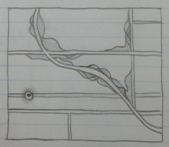
\includegraphics[scale=1]{figures/wire-1.png}
    \caption{Initial wireframe for histogram approach.}
    \label{fig:wire-1}
  \end{centering}
\end{figure}

\begin{figure}[htbp!]
  \begin{centering}
    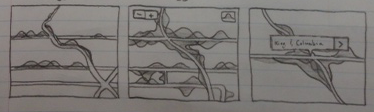
\includegraphics[scale=1]{figures/wire-2.png}
    \caption{Application wireframes showing interaction controls and pop-up menu.}
    \label{fig:wire-2}
  \end{centering}
\end{figure}

As can be seen in Figures \ref{fig:wire-1} - \ref{fig:wire-4}, various overlay techniques using both histograms and circular polygons on a map of a city were explored here in this early stage.
The histogram approach sought to model each vehicle (or small group of vehicles) on the road as a probability density function that could be moved along a road based on knowledge of traffic presence at each intersection, and speed limit data on each road.
More vehicles means more histograms, shown as translucent graphs which when overlaid, become more and more opaque, thus indicating a higher traffic density in that area.

\begin{figure}[htbp!]
  \begin{centering}
    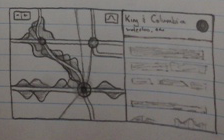
\includegraphics[scale=1]{figures/wire-4.png}
    \caption{Sketch of potential side menu for the Relay Interface application.}
    \label{fig:wire-3}
  \end{centering}
\end{figure}

Response for this concept was generally critical, as probability functions overlaid on a map were found to not be particularly easy to understand, at least not immediately at a glance.
It was evident at this stage that a simpler - more intuitive - visualization was needed for this application to be useful for both consumers and traffic engineers.

\begin{figure}[htbp!]
  \begin{centering}
    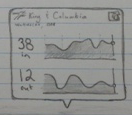
\includegraphics[scale=1]{figures/wire-5.png}
    \caption{Sketch of a detailed pop-up menu showing intersection data.}
    \label{fig:wire-4}
  \end{centering}
\end{figure}

Through exploration of the circular polygon heat-map concept, a more agreeable solution was found.
This concept modelled traffic data on a per intersection basis.
In other words, when an intersection is experiencing a high volume of traffic, a translucent circular polygon is triggered and overlaid onto a map of the city at the longitude and latitude of the intersection.
The size of the circle is positively correlated to the volume of traffic at the intersection.
A second degree of data is then shown through use of colour, to illustrate the performance of the intersection itself.
This gives insight into how well the intersection is moving traffic given it's high-volume state.
It was agreed upon that a well-performing high-volume intersection should receive a colour that is neutral, while a high-volume intersection with poor performance should emit a colour that indicates that something is wrong, such as orange or red.

It can also be seen in the figures that other components of the prototype application were accounted for in the wireframes.
These include interactions such as pop-up dialogues, highlighting routes and communicating intersections, as well as a side-panel for showing detailed metrics on intersection and overall city-wide traffic performance.
From this stage, the prototype moved to a mid-fidelity phase to further build out the concepts and refine the aesthetic of the application.

While not all of these early-stage concepts were used in the final product, the process of generating, critiquing, and refining multiple ideas proved valuable throughout the year.
These initial visualization concepts helped to spawn and guide future implementations, and helped attain a clear understanding of the data being presented.
The next step in the design process moved into a medium-fidelity stage, such that navigation and interaction could be explored at a deeper level.

\subsubsection{Medium-Fidelity Prototyping}
Through the use of prototyping software Balsamiq, a set of interactive mockups were created to both reflect the requirements of the application, as well as ideas and lessons learned from the previous wireframing stage.
In this prototype, the main tenets for the final version of the application were created in an illustrative form, to identify key architectural components and the user's interaction within.
By doing this in a medium that does not put too much focus on the specifics of visual design, it was easier to concentrate on the core features of the application, and how they satisfy (or dissatisfy) the original requirements. 

At this stage, the concept of data layers was explored.
Given that there are many varying metrics identified as important to target users (Traffic Engineers), and that these metrics all have a spatial or location-based relevance, the idea of turning on and off layers of data visualization overlaid on a map was critical in effectively demonstrating traffic data.
Metrics such as intersection Status, and Flow through an intersection were conceptualized at this stage, with some preliminary UI put together for interacting with these layers.
A screenshot of the mockup showing a Status visualization in the Relay app is presented in Figure \ref{fig:bals-1}. \\

\begin{figure}[htbp!]
  \begin{centering}
    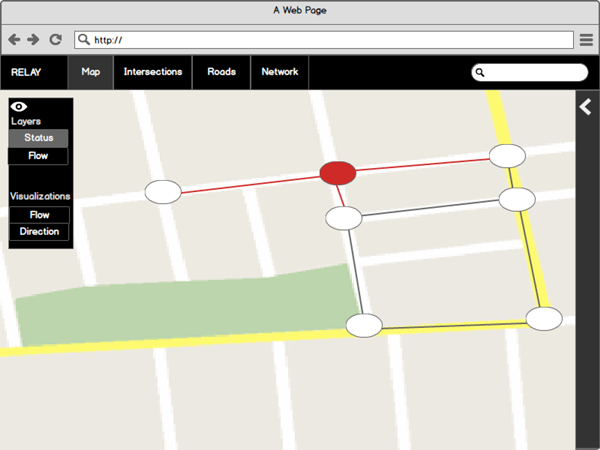
\includegraphics[scale=0.65]{figures/bals-1.png}
    \caption{Balsamiq mockup of a data layer in the Relay app.}
    \label{fig:bals-1}
  \end{centering}
\end{figure}

Additionally, as can be seen at the top of Figure \ref{fig:bals-1} the foundations for global app navigation were built out, in the form of a fixed header bar at the top of the screen.
This header serves many purposes, including branding for the app, search functionality, as well as tabbed buttons to move between contextually grouped pages.
Figure \ref{fig:bals-1} shows the active state of the Map button, while the main area of the screen contains a map with relevant data.

Further interaction design was carried out at this stage, in the form of a modular popup window, referred to as the Relay info box.
This info box was designed to present deeper metrics for an intersection, and appears when an intersection on the map is clicked.
This allows users to quickly inspect any intersection of interest and monitor time-series data in the context of a specific location.
Data provided at this stage includes a graph of the flow of traffic through the intersection in each of the cardinal directions, as well as a matching chart that provides predictive data into the near future, based on stochastic methods from the controller.
The status of the lights is shown, in addition to numerical car counts and the name of the intersection that has been clicked.
A Balsamiq mockup of the info box is presented in Figure \ref{fig:bals-2}. \\

\begin{figure}[htbp!]
  \begin{centering}
    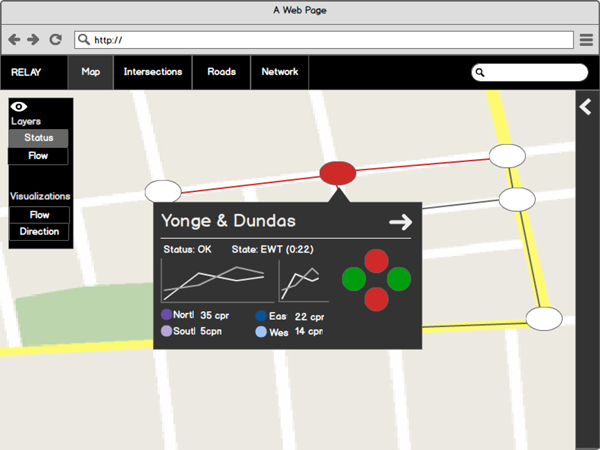
\includegraphics[scale=0.6]{figures/bals-2.png}
    \caption{Balsamiq mockup of the Relay info box.}
    \label{fig:bals-2}
  \end{centering}
\end{figure}

\begin{figure}[htbp!]
  \begin{centering}
    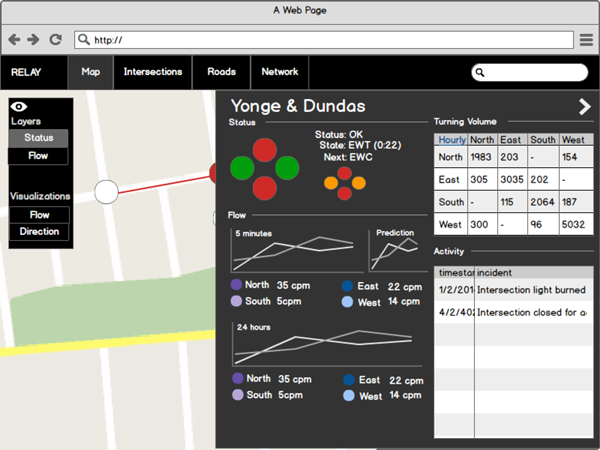
\includegraphics[scale=0.6]{figures/bals-3.png}
    \caption{Balsamiq mockup of the Relay dashboard.}
    \label{fig:bals-3}
  \end{centering}
\end{figure}

While the info box fulfills the need to browse intersections and provide quick snapshots of relevant intersection data, it was important for more advanced users to get an in depth look at this data, such that meaningful trends can be detected and acted upon.
It was necessary for these users - Traffic Engineers - to view metrics on intersection Location, Name, Type, State, In Flow, Out Flow, Predictions, and more.
To accommodate this large quantity of data, a dashboard was prototyped at this stage, setting a preliminary layout for each of the required metrics.
This dashboard slides across the screen from the right by pressing the arrow in the info box, and can then be toggled back and forth with the controls in the upper right corner of the screen.
A Balsamiq mockup of the dashboard can be found above in Figure \ref{fig:bals-3}.
As various intersections are selected on the map, the dashboard updates it's information to reflect that of the intended location.
Time-series graphs update in real-time as data feeds through the system, and an activity log hosts the history of noteworthy incidents at the selected intersection.

With these views on the Map screen prototyped in medium-fidelity, the design progressed into other areas of the application.
Moving through the global navigation buttons along the header, an Intersections page was mocked up.
The goal of this page is to give Traffic Engineers a holistic view on their network, as well as the ability to filter/search and target individual intersections.
This text-based search also allows for insight into any particular intersection by name, as well as the ability to find important groups of intersections or main arteries with many cross streets.
This is important because it allows users to locate intersections in two ways: spatially on the map, and now textually in the intersections table.
A mockup of the Intersections page is shown in Figure \ref{fig:bals-4}, with placeholder data in the intersections table. \\

\begin{figure}[htbp!]
  \begin{centering}
    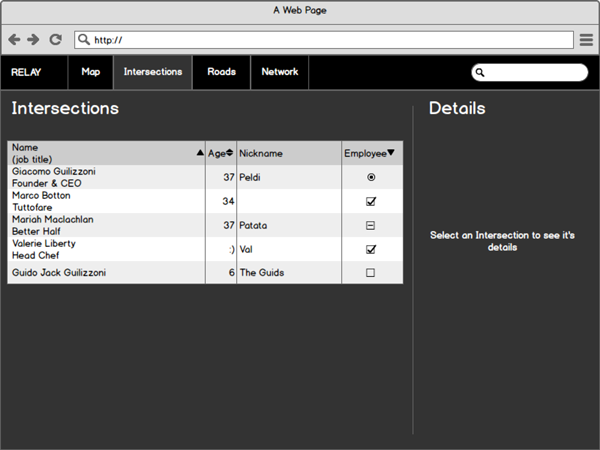
\includegraphics[scale=0.65]{figures/bals-4.png}
    \caption{Balsamiq mockup of the Intersections page.}
    \label{fig:bals-4}
  \end{centering}
\end{figure}

Finally, the medium-fidelity prototyping stage moved on to build out a layout and basic information for a Network page.
The intention of this page is to provide details similar to what would be shown in the info box or dashboard of an intersection, but for the entire network as a whole.
This allows Traffic Engineers to view, understand, diagnose, and make decisions for the network on a macro level, in addition to the finer look provided on a per intersection basis.
A mockup of the Network page is shown in Figure \ref{fig:bals-5}. \\

\begin{figure}[htbp!]
  \begin{centering}
    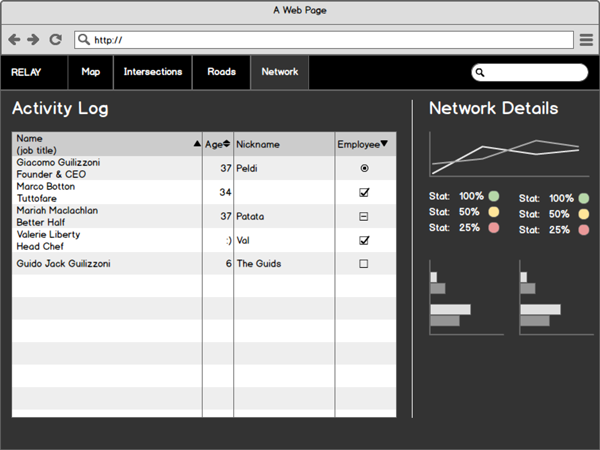
\includegraphics[scale=0.6]{figures/bals-5.png}
    \caption{Balsamiq mockup of the Network page.}
    \label{fig:bals-5}
  \end{centering}
\end{figure}

As can be seen in Figure \ref{fig:bals-5}, a large activity table is provided on the Network page, to highlight issues that occur at all intersections in the network.
These issues include accidents, power outages, abnormal volumes, and more.
Additional detail can be seen on the right hand side of the screen, with quantitative network data placed in charts and numerical tables, and colour-coding of network statuses explored at this stage.

Overall, the medium-fidelity prototyping stage was essential in moving the design of the Relay application forward towards its final state.
With functional requirements set in place, and now a strong roadmap of UI elements, navigation, page layout, and interactions to fulfill the requirements, the application was ready to be built in a high-fidelity form, as described in the following section.

\subsubsection{High-Fidelity Prototyping}
In preparation for the development of the Relay application, the design of the environment moved into a final high-fidelity prototyping phase.
This stage involved a major visual overhaul of the application, focusing on the definition of a unique design language to bring Relay together as a cohesive product.
Considerations at this stage include the creation of a custom grid structure, typography, colour, branding, the development of data visualization layers, and repurposing the search functionality in the app.
The high-fidelity design was done in Adobe Photoshop, Illustrator, and in the browser using HTML/CSS and JavaScript.
These tools allowed for highly accurate creation of assets, development of colour scheme, precise layout of visual elements, and more.

The branding for Relay was created in two main components: the logo, and the typesetting.
The logo is a custom glyph used in the application to denote the state of the signal at an intersection.
It contains four dots in a diamond pattern, with two fully-coloured dots positioned vertically, and two empty dots with a medium-weight stroke positioned horizontally.
In the application, this glyph would represent the flow of traffic in an East-West manner, while North-South traffic is halted at a red light.
This was selected to represent Relay as it both subtly represents what the application does, and provides important information to users in a modern and clean way.
The final Relay branding is shown in Figure \ref{fig:relay-logo}. \\ \\

\begin{figure}[htbp!]
  \begin{centering}
    
\includegraphics[scale=0.7]{figures/relay-logo.png}
    \caption{High-fidelity rendering of the Relay branding.}
    \label{fig:relay-logo}
  \end{centering}
\end{figure}

The typesetting was done to represent Relay in a way that would be clear, trustworthy, confident, readable, and modern.
The use of custom letter positioning through tracking and kerning methods aided this, while promoting clarity and confidence with the capitalization of each letter in the word.
Open Sans, a typeface that is freely available to the public, was utilized for the clean and readable aesthetic it provides.
As a sans-serif font set at a semi-bold weight, each letter is clear from any distance, at many sizes, on both screen and in print.
This also gives the branding a modern feel, as many serifed fonts are often associated with older, more classical and formal scenarios.

The high-fidelity design of the application itself began at a structural level, to set the basis for a consistent, coherent, and unique interface.
A grid structure was optimized for a 1440 x 900 pixel resolution screen - a common resolution on modern screens, and the dimensions of the screens used for the Symposium demo.
The grid was based upon units of 16 pixels, which was decided to be the lowest common denominator for icon and type sizing to ensure usability from many angles and distances.
With a grid structure in place, all following design decisions then had a reference point to follow from.
This aided in the purposeful use of negative spacing, symmetry, and balance of each screen composition.
The grid on a blank canvas is shown in Figure \ref{fig:dot-grid}. \\

\begin{figure}[htbp!]
  \begin{centering}
    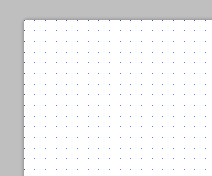
\includegraphics[scale=1]{figures/dot-grid.png}
    \caption{16 pixel grid foundation for the Relay user interface.}
    \label{fig:dot-grid}
  \end{centering}
\end{figure}

The first consideration in developing the design language for the application was the typography.
Just like the branding, the typography was intended to be clear and readable, but also neutral in tone.
Neutrality of the type allows for clear representation of the content itself, which is highly important in such a data-heavy application.
As a critical element of the user interface, particular attention was paid to hierarchy of type sizes and weights, all deriving from a smallest line-height of 16 pixels, used in small data labels and body.
The typeface Helvetica Neue was used, as it is well-known to provide very clear and readable text at many sizes, with a neutral tone.
Additionally, it is a common typeface used in the signage of many major cities around the world.
This gives the application a recognizable and associative feeling, which is especially important for an application that deals with traffic conditions in urban areas.
An example of an intersection name set in 24pt Helvetica Neue Bold is shown in Figure \ref{fig:name}. \\

\begin{figure}[htbp!]
  \begin{centering}
    
\includegraphics[scale=1]{figures/name.png}
    \caption{An intersection name set in 24pt Helvetica Neue Bold.}
    \label{fig:name}
  \end{centering}
\end{figure}

The high-fidelity prototyping process continued with the development of colour-scheme for the application.
Given the importance of visualizing data in the Relay app, it was decided that all non-data elements of the UI - the map, modular overlays, and header, for example - should be subdued and clearly grouped together as functionally similar elements.
To accomplish this, a black and white UI was established for all control elements, providing a clean environment for navigation, while vibrant, highly-saturated colours were used for charts and data layers.
This technique effectively created a high-contrast environment where areas that require visual focus, attention, and thought - i.e. the data - were the most salient elements on the screen, and any layout or navigational components were done in a clear black and white manner, similar to signage found on the streets of many major cities.
Therefore, all contextually similar elements were easily grouped and identifiable through their similarities or differences in colour.
An example of a chart showing the flow of traffic through an intersection over time is illustrated in Figure \ref{fig:chart}.
Notice the vibrancy of the coloured data, and its contrast with the structural page elements surrounding it. \\

\begin{figure}[htbp!]
  \begin{centering}
    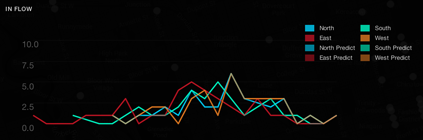
\includegraphics[scale=0.9]{figures/chart.png}
    \caption{A chart showing the flow of traffic through an intersection over time.}
    \label{fig:chart}
  \end{centering}
\end{figure}

The data visualization layers were next to be developed at the high-fidelity stage.
These visualizations took the form of heat maps, as well as quantitative, relative, and boolean glyphs, representing data on the Status, Flow, and Queue Length at a given intersection.
The first visualization layer, showing the Status of intersections, used small dot glyphs of different colour to display the boolean status of a light.
By overlaying a dot at each intersection, with a corresponding white or red colour to denote proper working condition vs. an error, such as a power outage, an easily digestible visualization was created.
This empowers Traffic Engineers to easily monitor their network, and to detect any anomalies that may have occurred.
A screenshot of the Status layer is shown in Figure \ref{fig:status}. \\

\begin{figure}[htbp!]
  \begin{centering}
    
\includegraphics[scale=0.9]{figures/status.png}
    \caption{A screenshot of the intersection Status data layer.}
    \label{fig:status}
  \end{centering}
\end{figure}

The second data layer to be designed was a heat map representing the flow of traffic through intersections.
This was accomplished on a per-intersection basis, and was intended to provide a macro view of the relative traffic density across areas of the city.
This view is most useful for those looking for an overview of general traffic conditions, such as a browsing Traffic Engineer, or a consumer looking to plan a route through the city.
A screenshot of the first Flow visualization layer is shown in Figure \ref{fig:flow-1}.

\begin{figure}[htbp!]
  \begin{centering}
    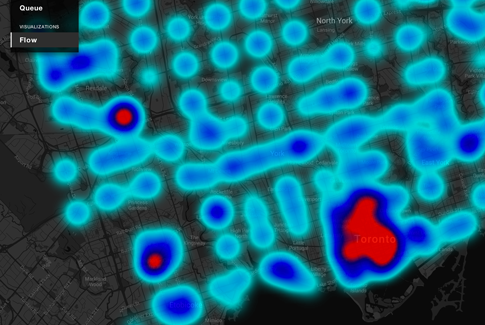
\includegraphics[scale=0.9]{figures/flow-1.png}
    \caption{A screenshot of the flow per-intersection heat map.}
    \label{fig:flow-1}
  \end{centering}
\end{figure}

Following this Flow visualization, a second implementation of traffic flow was developed, this time looking at flow between intersections, rather than at or through any particular intersection.
This was accomplished by taking predictive data from the controller, and approximating the position of cars along roadways given the knowledge of their entry and exit directions from each intersection.
Each car is plotted as a low-opacity glyph of concentric circles, with a bright green core, a lighter green exterior, and a soft blue outline, denoting the estimated nature of the position of any given car.
Given the large number of vehicles to be accounted for, a low opacity was selected for each individual glyph, so that as they overlap with one another, the intensity of the colour increases so as to illustrate the increasing density of traffic in an area.
A screenshot of the Flow between intersections data layer is shown in Figure \ref{fig:flow-2}.

\begin{figure}[htbp!]
  \begin{centering}
    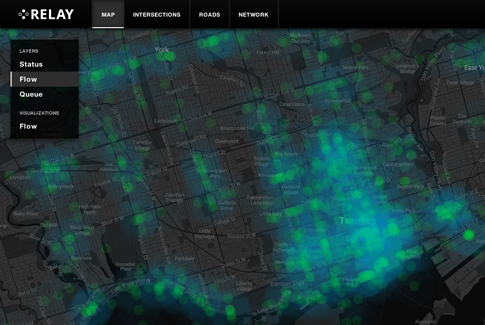
\includegraphics[scale=0.9]{figures/flow-2.png}
    \caption{A screenshot of the flow between intersections heat map.}
    \label{fig:flow-2}
  \end{centering}
\end{figure}

As can be seen in Figure \ref{fig:flow-2}, the natural visualization of major roadways and arteries through the cities is evident, which is an important result of this visualization.
A wide range of traffic patterns can be derived from this, thanks to the high-resolution of data points that give a continuous feel to the data, as opposed to the limited two-stage discrete options currently available through applications such as Google and Apple Maps.

Finally, the final visualization layer looked to showcase the data representing Queue Length or average wait time at an intersection.
The goal of this visualization was to produce glyphs that could show both quantitative measures, as well as give a sense of relative weighting between intersections.
A four-pronged glyph was developed, with three short prongs extending in the East, South, and West directions, while a variably sized prong extends to the North.
The length of the North prong corresponds to the average wait time at a given intersection, while the three shorter prongs are of equal length and serve as a stand for the quantitative North measure.
This creates a pseudo 3-dimensional effect, and gives the user a unique look at the changing landscape of queue lengths in the city - similar to how a city skyline may look with many tall buildings.
A screenshot of the Queue Length visualization layer is shown in Figure \ref{fig:queue}.

\begin{figure}[htbp!]
  \begin{centering}
    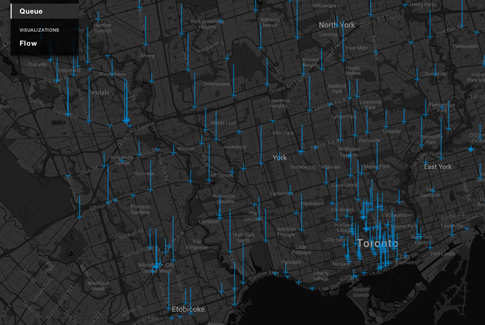
\includegraphics[scale=0.9]{figures/queue.png}
    \caption{A screenshot of the average queue length at each intersection.}
    \label{fig:queue}
  \end{centering}
\end{figure}

Following the design of the data visualization layers, the high-fidelity stage looked at the search functionality of the application, and focused attention on repurposing its form to better reflect its function.
Previous prototypes held the search bar in the header across all pages of the application.
This proved to be troublesome, as some pages did not require any search functionality, while the ones that did actually served as text-based filters within the context of the current page.
The high-fidelity design saw the removal of the search bar from the global navigation header, and into the upper section of the Intersections and Network pages.
This way, the text-based tables found on these pages could be easily searched/filtered, without the confusion of entering text into the global header, where a new page would be the expected result.

An additional feature that made its way through the high-fidelity phase is the Connection Status window.
This window is activated through the gear icon in the top right corner of the screen, and is useful for monitoring the status of the connection between the front-end and back-end of the application.
This window is positioned in the top-right of the screen so as to avoid covering any important visual elements, and is padded in from the top and right sides of the screen to maintain access to the dashboard toggle button.
The connection status window identifies where the data is coming from: either through a Web Socket or through the application's REST API.
It also identifies time since the last data update, both locally on a selected intersection, and globally over the entire network.
A screenshot of the Connection Status window is shown in Figure \ref{fig:connection}.

\begin{figure}[htbp!]
  \begin{centering}
    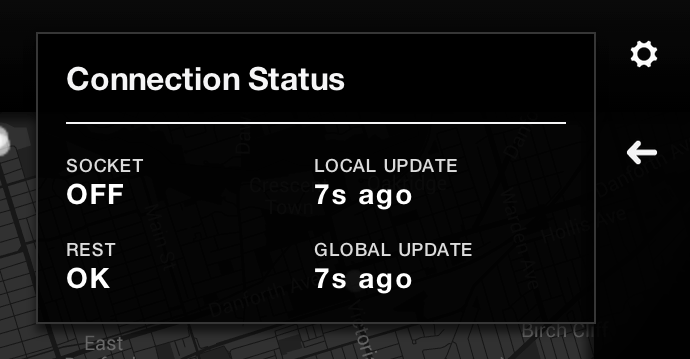
\includegraphics[scale=0.6]{figures/connection.png}
    \caption{A screenshot of the connection status window.}
    \label{fig:connection}
  \end{centering}
\end{figure}

Lastly, the intersection dashboard was refined at a high-fidelity stage.
The specific metrics contained in the dashboard were iterated on and refined from the medium-fidelity stage to accurately reflect the data coming from the back-end controller.
This involved splitting the Flow metric into In-Flow and Out-Flow at an intersection, showing the current and next intended State of the traffic lights, and providing a new Turn Predictions matrix, which gives the predicted quantity of cars moving through each permutation of turns based on stochastic data from the back-end.
In-line with the medium-fidelity prototype, the Activity Log is provided giving consideration to readability and interaction, with subtle hover states on individual table rows to improve salience of desired fields.
Additional information includes the Intersection ID and the Intersection Type, two identifiers that are often important to Traffic Engineers.
A screenshot of the high-fidelity dashboard is shown in Figure \ref{fig:dashboardt}. \\

\begin{figure}[htbp!]
  \begin{centering}
    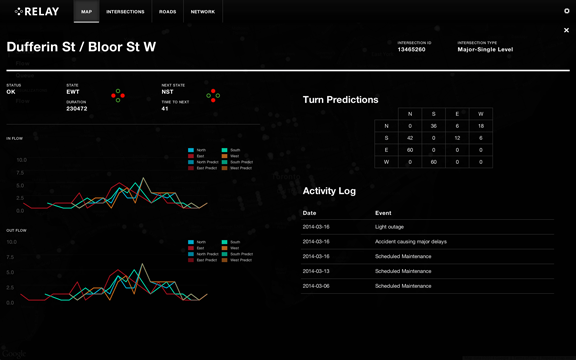
\includegraphics[scale=0.73]{figures/dashboard.png}
    \caption{A screenshot of the Relay intersection dashboard.}
    \label{fig:dashboardt}
  \end{centering}
\end{figure}

With these elements in place, the final developmental/functional touches to the Relay application were ready to be built for the demo, as showcased on Symposium day.
As a unit, the application is held together using the modular design elements described above, which makes the application easily scalable and modifiable for individual implementations or changing metrics and requirements.
With a unique and well-defined design language established, further extrapolations of this implementation have a library of best practices and UI elements that can be carried forward into new scenarios.

\subsection{Application Architecture}

Application interfaces for critical infrastructure must be highly robust and reliable. Furthermore, it is important the the systems are able to scale in order to accomodate the inevitable growth of the system. These main ideas drove the design of the front-end (web application) application architecture. 

Given the breadth of choices in software technology, it was necessary to use a quantifiable selection process for determining the appropriate solutions from a group of candidates. The three main areas of the front-end application which required such a process are the Framework, Mapping Library, and Visualization Library. The selection process for these is discussed in the following sections.

\subsubsection{Framework Selection}

Software frameworks are code libraries which provide functionality that enables developers to more easily implement a specific software pattern. One of the most common software patterns is the Model-View-Controller (MVC) pattern, which is commonly used in complex and large software applications to ensure the application is reliable, structured, and can scale effectively. Similarly, front-end software frameworks allows for the development of structered and scalable applications by providing software pattern untilities. Given the critical nature of our application, it was determined that the use of a framework would be appropriate for ensuring the scalability and reliabilty of the application.

Four JavaScript frameworks were selected for comparison. Javascript MVC is a mature, well-known front-end MVC implementation which is build off of jQuery, a JavaScript Utility Library, which offers a well-rounded feature base. DOJO is another mature and well-known framework which does not offer an MVC-style framework, yet is class-oriented. Backbone.JS is a relatively new Model-View (MV) framework built off of the Underscore.js utility library. Finally, Angular.js is a new and highly functional front-end framework which loosely follows an MVC pattern.

The frameworks are scored across five weighted features. The scores are justified and a winning framework is selected.

\begin{enumerate}

\item \textbf{Size} - The use of large JavaScript libraries can cause performance issues within the application. The selected library should be as small as possible. Candidate frameworks will be assesed based on the size of their encompassing code files. This feature has been given a weight of 0.5.

\item \textbf{Independance} - The selected framework should be self-contained and not require many prerequisite JavaScript Libraries in order to function. The presence of many prerequisite libraries increases the size of the application and will slow down performance. Candidate frameworks are assesed based on the number of prerequisite frameworks and plug-ins required for the framework's application within the proposed solution. This feature has been given a weight of 0.5.

\item \textbf{Functionality} - The selected JavaScript framework should provide a rich set functionality which is not available within the native Javascript language. Important functionality includes utility functions, templating, Document Object Model (DOM) binding, client-server communication methods, and data structure classes. Candidate frameworks are assessed based on the both the quantity and quality of the functionality provided, in the context of the proposed soluction. This feature has been given a weight of 0.8, as it is important that the framework provide sufficient functionality to implement the solution.

\item \textbf{Modularity} - It is important that the selected JavaScvript framework supports the creation of modular code, given the complexity of the proposed solution. The selected MVC framework should encourage an exablished code pattern, such as and MV- or MVC-style structure. Candidate frameworks are assesed based on their similarity to known software architecture patterns, such as MV or MVC. Due to the importance of scalability and modularity in the proposed solution, this feature has been given a weighting of 0.8.

\item \textbf{Implementation Overhead} - The selected JavaScript framework should not require excessive amounts of overhead code in order to successfully suit the needs of the proposed solution. The selected framework should have as little overhead as possible. Candidate frameworks are assessed by examining tutorial code implementations for each framework, to determine the proportion of development required as overhead compared to application-specific code. This feature has been given a weight of 0.5.

\end{enumerate}

The frameworks are presented in a weighted decision matrix below. Each attribute is weighted out of 5 points for each of the candidate frameworks. Weightings for each a.







\end{document}